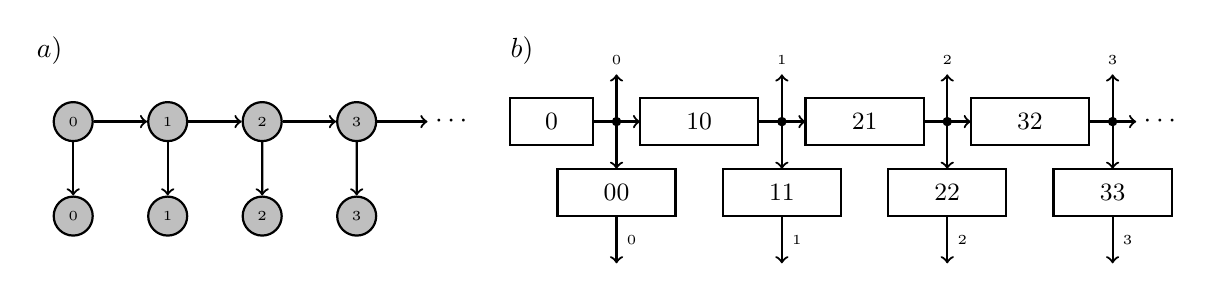
\begin{tikzpicture}[scale=0.3,thick] % , baseline = -3.5pt

\node[anchor=center] (text) at (-1,3) {${a)}$};

	\node [circle, draw, thick, fill=gray!50] (T1) at (0,0) {\tiny $\catvariableof{0}$};
	\node [circle, draw, thick, fill=gray!50] (E1) at (0,-4) {\tiny $\randomeof{0}$};
	\draw[->] (T1) -- (E1);	
	\node [circle, draw, thick, fill=gray!50] (T2) at (4,0) {\tiny $\catvariableof{1}$};
	\node [circle, draw, thick, fill=gray!50] (E2) at (4,-4) {\tiny $\randomeof{1}$};
	\draw[->] (T2) -- (E2);	
	\draw[->] (T1) -- (T2);	
	\node [circle, draw, thick, fill=gray!50] (T3) at (8,0) {\tiny $\catvariableof{2}$};
	\node [circle, draw, thick, fill=gray!50] (E3) at (8,-4) {\tiny $\randomeof{2}$};
	\draw[->] (T3) -- (E3);	
	\draw[->] (T2) -- (T3);
	\node [circle, draw, thick, fill=gray!50] (T4) at (12,0) {\tiny $\catvariableof{3}$};
	\node [circle, draw, thick, fill=gray!50] (E4) at (12,-4) {\tiny $\randomeof{3}$};
	\draw[->] (T4) -- (E4);	
	\draw[->] (T3) -- (T4);
	\draw[->] (T4) -- (15,0);

	\node[anchor=center] (text) at (16,0) {$\cdots$};

	%\node [circle, draw, thick, fill=gray!50] (T4) at (17,0) {\tiny $\catvariableof{\atomorder}$};
	%\draw[->] (14,0) -- (T4);	
			

\begin{scope}[shift={(22,0)}]

\node[anchor=center] (text) at (-3,3) {${b)}$};

\draw (-3.5,-1) rectangle (0, 1);
\node[anchor=center] (text) at (-1.75,0) {\small $\probat{\catvariableof{0}}$};
\draw[->] (0,0) -- (2,0);
\draw[fill] (1,0) circle (0.15cm);
\draw[->] (1,0) -- (1,2) node[above] {\tiny ${\catvariableof{0}}$};
\draw[->] (1,0) -- (1,-2);
\draw (-1.5,-2) rectangle (3.5,-4); 
\node[anchor=center] (text) at (1,-3) {\small $\condprobof{\randomeof{0}}{\catvariableof{0}}$};
\draw[->] (1,-4) -- (1,-6) node[midway, right]{\tiny ${\randomeof{0}}$};

\draw (2,-1) rectangle (7, 1);
\node[anchor=center] (text) at (4.5,0) {\small $\condprobof{\catvariableof{1}}{\catvariableof{0}}$};
\draw[->]  (7,0) -- (9,0);
\draw[fill] (8,0) circle (0.15cm);
\draw[->] (8,0) -- (8,2) node[above] {\tiny ${\catvariableof{1}}$};
\draw[->] (8,0) -- (8,-2);
\draw (5.5,-2) rectangle (10.5,-4); 
\node[anchor=center] (text) at (8,-3) {\small $\condprobof{\randomeof{1}}{\catvariableof{1}}$};
\draw[->] (8,-4) -- (8,-6) node[midway, right]{\tiny ${\randomeof{1}}$};


\draw (9,-1) rectangle (14, 1);
\node[anchor=center] (text) at (11.5,0) {\small $\condprobof{\catvariableof{2}}{\catvariableof{1}}$};
\draw[->]  (14,0) -- (16,0);
\draw[fill] (15,0) circle (0.15cm);
\draw[->] (15,0) -- (15,2) node[above] {\tiny ${\catvariableof{2}}$};
\draw[->] (15,0) -- (15,-2);
\draw (12.5,-2) rectangle (17.5,-4); 
\node[anchor=center] (text) at (15,-3) {\small $\condprobof{\randomeof{2}}{\catvariableof{2}}$};
\draw[->] (15,-4) -- (15,-6) node[midway, right]{\tiny ${\randomeof{2}}$};

\draw (16,-1) rectangle (21, 1);
\node[anchor=center] (text) at (18.5,0) {\small $\condprobof{\catvariableof{3}}{\catvariableof{2}}$};
\draw[->]  (21,0) -- (23,0);
\draw[fill] (22,0) circle (0.15cm);
\draw[->] (22,0) -- (22,2) node[above] {\tiny ${\catvariableof{3}}$};
\draw[->] (22,0) -- (22,-2);
\draw (19.5,-2) rectangle (24.5,-4); 
\node[anchor=center] (text) at (22,-3) {\small $\condprobof{\randomeof{3}}{\catvariableof{3}}$};
\draw[->] (22,-4) -- (22,-6) node[midway, right]{\tiny ${\randomeof{3}}$};


\node[anchor=center] (text) at (24,0) {$\cdots$};


\end{scope}

\end{tikzpicture} 